\documentclass[1p]{elsarticle_modified}
%\bibliographystyle{elsarticle-num}

%\usepackage[colorlinks]{hyperref}
%\usepackage{abbrmath_seonhwa} %\Abb, \Ascr, \Acal ,\Abf, \Afrak
\usepackage{amsfonts}
\usepackage{amssymb}
\usepackage{amsmath}
\usepackage{amsthm}
\usepackage{scalefnt}
\usepackage{amsbsy}
\usepackage{kotex}
\usepackage{caption}
\usepackage{subfig}
\usepackage{color}
\usepackage{graphicx}
\usepackage{xcolor} %% white, black, red, green, blue, cyan, magenta, yellow
\usepackage{float}
\usepackage{setspace}
\usepackage{hyperref}

\usepackage{tikz}
\usetikzlibrary{arrows}

\usepackage{multirow}
\usepackage{array} % fixed length table
\usepackage{hhline}

%%%%%%%%%%%%%%%%%%%%%
\makeatletter
\renewcommand*\env@matrix[1][\arraystretch]{%
	\edef\arraystretch{#1}%
	\hskip -\arraycolsep
	\let\@ifnextchar\new@ifnextchar
	\array{*\c@MaxMatrixCols c}}
\makeatother %https://tex.stackexchange.com/questions/14071/how-can-i-increase-the-line-spacing-in-a-matrix
%%%%%%%%%%%%%%%

\usepackage[normalem]{ulem}

\newcommand{\msout}[1]{\ifmmode\text{\sout{\ensuremath{#1}}}\else\sout{#1}\fi}
%SOURCE: \msout is \stkout macro in https://tex.stackexchange.com/questions/20609/strikeout-in-math-mode

\newcommand{\cancel}[1]{
	\ifmmode
	{\color{red}\msout{#1}}
	\else
	{\color{red}\sout{#1}}
	\fi
}

\newcommand{\add}[1]{
	{\color{blue}\uwave{#1}}
}

\newcommand{\replace}[2]{
	\ifmmode
	{\color{red}\msout{#1}}{\color{blue}\uwave{#2}}
	\else
	{\color{red}\sout{#1}}{\color{blue}\uwave{#2}}
	\fi
}

\newcommand{\Sol}{\mathcal{S}} %segment
\newcommand{\D}{D} %diagram
\newcommand{\A}{\mathcal{A}} %arc


%%%%%%%%%%%%%%%%%%%%%%%%%%%%%5 test

\def\sl{\operatorname{\textup{SL}}(2,\Cbb)}
\def\psl{\operatorname{\textup{PSL}}(2,\Cbb)}
\def\quan{\mkern 1mu \triangleright \mkern 1mu}

\theoremstyle{definition}
\newtheorem{thm}{Theorem}[section]
\newtheorem{prop}[thm]{Proposition}
\newtheorem{lem}[thm]{Lemma}
\newtheorem{ques}[thm]{Question}
\newtheorem{cor}[thm]{Corollary}
\newtheorem{defn}[thm]{Definition}
\newtheorem{exam}[thm]{Example}
\newtheorem{rmk}[thm]{Remark}
\newtheorem{alg}[thm]{Algorithm}

\newcommand{\I}{\sqrt{-1}}
\begin{document}

%\begin{frontmatter}
%
%\title{Boundary parabolic representations of knots up to 8 crossings}
%
%%% Group authors per affiliation:
%\author{Yunhi Cho} 
%\address{Department of Mathematics, University of Seoul, Seoul, Korea}
%\ead{yhcho@uos.ac.kr}
%
%
%\author{Seonhwa Kim} %\fnref{s_kim}}
%\address{Center for Geometry and Physics, Institute for Basic Science, Pohang, 37673, Korea}
%\ead{ryeona17@ibs.re.kr}
%
%\author{Hyuk Kim}
%\address{Department of Mathematical Sciences, Seoul National University, Seoul 08826, Korea}
%\ead{hyukkim@snu.ac.kr}
%
%\author{Seokbeom Yoon}
%\address{Department of Mathematical Sciences, Seoul National University, Seoul, 08826,  Korea}
%\ead{sbyoon15@snu.ac.kr}
%
%\begin{abstract}
%We find all boundary parabolic representation of knots up to 8 crossings.
%
%\end{abstract}
%\begin{keyword}
%    \MSC[2010] 57M25 
%\end{keyword}
%
%\end{frontmatter}

%\linenumbers
%\tableofcontents
%
\newcommand\colored[1]{\textcolor{white}{\rule[-0.35ex]{0.8em}{1.4ex}}\kern-0.8em\color{red} #1}%
%\newcommand\colored[1]{\textcolor{white}{ #1}\kern-2.17ex	\textcolor{white}{ #1}\kern-1.81ex	\textcolor{white}{ #1}\kern-2.15ex\color{red}#1	}

{\Large $\underline{12a_{0399}~(K12a_{0399})}$}

\setlength{\tabcolsep}{10pt}
\renewcommand{\arraystretch}{1.6}
\vspace{1cm}\begin{tabular}{m{100pt}>{\centering\arraybackslash}m{274pt}}
\multirow{5}{120pt}{
	\centering
	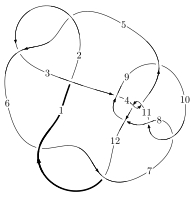
\includegraphics[width=112pt]{../../../GIT/diagram.site/Diagrams/png/1200_12a_0399.png}\\
\ \ \ A knot diagram\footnotemark}&
\allowdisplaybreaks
\textbf{Linearized knot diagam} \\
\cline{2-2}
 &
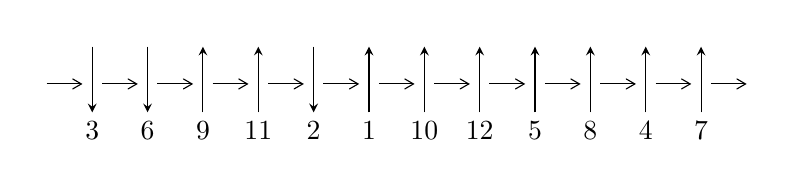
\begin{tikzpicture}[x=20pt, y=17pt]
	% nodes
	\node (C0) at (0, 0) {};
	\node (C1) at (1, 0) {};
	\node (C1U) at (1, +1) {};
	\node (C1D) at (1, -1) {3};

	\node (C2) at (2, 0) {};
	\node (C2U) at (2, +1) {};
	\node (C2D) at (2, -1) {6};

	\node (C3) at (3, 0) {};
	\node (C3U) at (3, +1) {};
	\node (C3D) at (3, -1) {9};

	\node (C4) at (4, 0) {};
	\node (C4U) at (4, +1) {};
	\node (C4D) at (4, -1) {11};

	\node (C5) at (5, 0) {};
	\node (C5U) at (5, +1) {};
	\node (C5D) at (5, -1) {2};

	\node (C6) at (6, 0) {};
	\node (C6U) at (6, +1) {};
	\node (C6D) at (6, -1) {1};

	\node (C7) at (7, 0) {};
	\node (C7U) at (7, +1) {};
	\node (C7D) at (7, -1) {10};

	\node (C8) at (8, 0) {};
	\node (C8U) at (8, +1) {};
	\node (C8D) at (8, -1) {12};

	\node (C9) at (9, 0) {};
	\node (C9U) at (9, +1) {};
	\node (C9D) at (9, -1) {5};

	\node (C10) at (10, 0) {};
	\node (C10U) at (10, +1) {};
	\node (C10D) at (10, -1) {8};

	\node (C11) at (11, 0) {};
	\node (C11U) at (11, +1) {};
	\node (C11D) at (11, -1) {4};

	\node (C12) at (12, 0) {};
	\node (C12U) at (12, +1) {};
	\node (C12D) at (12, -1) {7};
	\node (C13) at (13, 0) {};

	% arrows
	\draw[->,>={angle 60}]
	(C0) edge (C1) (C1) edge (C2) (C2) edge (C3) (C3) edge (C4) (C4) edge (C5) (C5) edge (C6) (C6) edge (C7) (C7) edge (C8) (C8) edge (C9) (C9) edge (C10) (C10) edge (C11) (C11) edge (C12) (C12) edge (C13) ;	\draw[->,>=stealth]
	(C1U) edge (C1D) (C2U) edge (C2D) (C3D) edge (C3U) (C4D) edge (C4U) (C5U) edge (C5D) (C6D) edge (C6U) (C7D) edge (C7U) (C8D) edge (C8U) (C9D) edge (C9U) (C10D) edge (C10U) (C11D) edge (C11U) (C12D) edge (C12U) ;
	\end{tikzpicture} \\
\hhline{~~} \\& 
\textbf{Solving Sequence} \\ \cline{2-2} 
 &
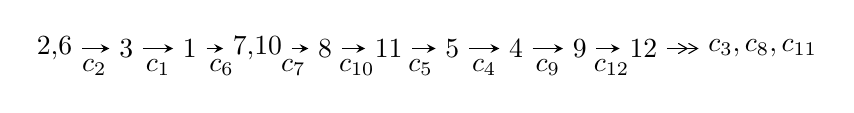
\begin{tikzpicture}[x=23pt, y=7pt]
	% node
	\node (A0) at (-1/8, 0) {2,6};
	\node (A1) at (1, 0) {3};
	\node (A2) at (2, 0) {1};
	\node (A3) at (49/16, 0) {7,10};
	\node (A4) at (33/8, 0) {8};
	\node (A5) at (41/8, 0) {11};
	\node (A6) at (49/8, 0) {5};
	\node (A7) at (57/8, 0) {4};
	\node (A8) at (65/8, 0) {9};
	\node (A9) at (73/8, 0) {12};
	\node (C1) at (1/2, -1) {$c_{2}$};
	\node (C2) at (3/2, -1) {$c_{1}$};
	\node (C3) at (5/2, -1) {$c_{6}$};
	\node (C4) at (29/8, -1) {$c_{7}$};
	\node (C5) at (37/8, -1) {$c_{10}$};
	\node (C6) at (45/8, -1) {$c_{5}$};
	\node (C7) at (53/8, -1) {$c_{4}$};
	\node (C8) at (61/8, -1) {$c_{9}$};
	\node (C9) at (69/8, -1) {$c_{12}$};
	\node (A10) at (11, 0) {$c_{3},c_{8},c_{11}$};

	% edge
	\draw[->,>=stealth]	
	(A0) edge (A1) (A1) edge (A2) (A2) edge (A3) (A3) edge (A4) (A4) edge (A5) (A5) edge (A6) (A6) edge (A7) (A7) edge (A8) (A8) edge (A9) ;
	\draw[->>,>={angle 60}]	
	(A9) edge (A10);
\end{tikzpicture} \\ 

\end{tabular} \\

\footnotetext{
The image of knot diagram is generated by the software ``\textbf{Draw programme}" developed by Andrew Bartholomew(\url{http://www.layer8.co.uk/maths/draw/index.htm\#Running-draw}), where we modified some parts for our purpose(\url{https://github.com/CATsTAILs/LinksPainter}).
}\phantom \\ \newline 
\centering \textbf{Ideals for irreducible components\footnotemark of $X_{\text{par}}$} 
 
\begin{align*}
I^u_{1}&=\langle 
8.68978\times10^{61} u^{110}-9.97257\times10^{61} u^{109}+\cdots+4.56538\times10^{61} b-5.74038\times10^{61},\\
\phantom{I^u_{1}}&\phantom{= \langle  }1.13849\times10^{61} u^{110}-5.27519\times10^{61} u^{109}+\cdots+4.56538\times10^{61} a+4.37740\times10^{61},\;u^{111}-2 u^{110}+\cdots-3 u^2+1\rangle \\
I^u_{2}&=\langle 
14 u^5+12 u^4-6 u^3-15 u^2+17 b-10 u-4,\;13 u^5+16 u^4-8 u^3-20 u^2+17 a-2 u+6,\\
\phantom{I^u_{2}}&\phantom{= \langle  }u^6+u^5- u^4-2 u^3+u+1\rangle \\
\\
\end{align*}
\raggedright * 2 irreducible components of $\dim_{\mathbb{C}}=0$, with total 117 representations.\\
\footnotetext{All coefficients of polynomials are rational numbers. But the coefficients are sometimes approximated in decimal forms when there is not enough margin.}
\newpage
\renewcommand{\arraystretch}{1}
\centering \section*{I. $I^u_{1}= \langle 8.69\times10^{61} u^{110}-9.97\times10^{61} u^{109}+\cdots+4.57\times10^{61} b-5.74\times10^{61},\;1.14\times10^{61} u^{110}-5.28\times10^{61} u^{109}+\cdots+4.57\times10^{61} a+4.38\times10^{61},\;u^{111}-2 u^{110}+\cdots-3 u^2+1 \rangle$}
\flushleft \textbf{(i) Arc colorings}\\
\begin{tabular}{m{7pt} m{180pt} m{7pt} m{180pt} }
\flushright $a_{2}=$&$\begin{pmatrix}1\\0\end{pmatrix}$ \\
\flushright $a_{6}=$&$\begin{pmatrix}0\\u\end{pmatrix}$ \\
\flushright $a_{3}=$&$\begin{pmatrix}1\\u^2\end{pmatrix}$ \\
\flushright $a_{1}=$&$\begin{pmatrix}- u^2+1\\- u^4\end{pmatrix}$ \\
\flushright $a_{7}=$&$\begin{pmatrix}u^5-2 u^3+u\\u^7- u^5+u\end{pmatrix}$ \\
\flushright $a_{10}=$&$\begin{pmatrix}-0.249374 u^{110}+1.15548 u^{109}+\cdots+1.33102 u-0.958826\\-1.90341 u^{110}+2.18439 u^{109}+\cdots+2.65883 u+1.25737\end{pmatrix}$ \\
\flushright $a_{8}=$&$\begin{pmatrix}0.372838 u^{110}+0.358652 u^{109}+\cdots+0.368291 u-1.43345\\-1.46447 u^{110}+1.53387 u^{109}+\cdots+3.34613 u+0.846984\end{pmatrix}$ \\
\flushright $a_{11}=$&$\begin{pmatrix}-2.54332 u^{110}+3.45704 u^{109}+\cdots+3.89125 u+2.46522\\-1.84245 u^{110}+2.92307 u^{109}+\cdots+1.27372 u+2.34650\end{pmatrix}$ \\
\flushright $a_{5}=$&$\begin{pmatrix}u\\u\end{pmatrix}$ \\
\flushright $a_{4}=$&$\begin{pmatrix}-0.265304 u^{110}-1.25314 u^{109}+\cdots-2.83145 u-2.31909\\-1.03887 u^{110}+0.341895 u^{109}+\cdots-2.01617 u-0.317190\end{pmatrix}$ \\
\flushright $a_{9}=$&$\begin{pmatrix}1.60670 u^{110}-1.55222 u^{109}+\cdots-0.323016 u-3.23798\\-0.0473347 u^{110}-0.523306 u^{109}+\cdots+1.00479 u-1.02178\end{pmatrix}$ \\
\flushright $a_{12}=$&$\begin{pmatrix}- u^8+3 u^6-3 u^4+1\\- u^{10}+2 u^8- u^6-2 u^4+u^2\end{pmatrix}$\\&\end{tabular}
\flushleft \textbf{(ii) Obstruction class $= -1$}\\~\\
\flushleft \textbf{(iii) Cusp Shapes $= 9.59749 u^{110}-11.8018 u^{109}+\cdots-18.8679 u-4.76652$}\\~\\
\newpage\renewcommand{\arraystretch}{1}
\flushleft \textbf{(iv) u-Polynomials at the component}\newline \\
\begin{tabular}{m{50pt}|m{274pt}}
Crossings & \hspace{64pt}u-Polynomials at each crossing \\
\hline $$\begin{aligned}c_{1}\end{aligned}$$&$\begin{aligned}
&u^{111}+60 u^{110}+\cdots+6 u+1
\end{aligned}$\\
\hline $$\begin{aligned}c_{2},c_{5}\end{aligned}$$&$\begin{aligned}
&u^{111}+2 u^{110}+\cdots+3 u^2-1
\end{aligned}$\\
\hline $$\begin{aligned}c_{3}\end{aligned}$$&$\begin{aligned}
&u^{111}- u^{110}+\cdots-44608 u-18496
\end{aligned}$\\
\hline $$\begin{aligned}c_{4},c_{11}\end{aligned}$$&$\begin{aligned}
&u^{111}-2 u^{110}+\cdots+4 u-1
\end{aligned}$\\
\hline $$\begin{aligned}c_{6},c_{12}\end{aligned}$$&$\begin{aligned}
&u^{111}+6 u^{110}+\cdots-2040 u-117
\end{aligned}$\\
\hline $$\begin{aligned}c_{7},c_{10}\end{aligned}$$&$\begin{aligned}
&u^{111}+7 u^{110}+\cdots-4863 u-289
\end{aligned}$\\
\hline $$\begin{aligned}c_{8}\end{aligned}$$&$\begin{aligned}
&17(17 u^{111}+139 u^{110}+\cdots-2325314 u-254971)
\end{aligned}$\\
\hline $$\begin{aligned}c_{9}\end{aligned}$$&$\begin{aligned}
&17(17 u^{111}+141 u^{110}+\cdots+7037007 u-1137879)
\end{aligned}$\\
\hline
\end{tabular}\\~\\
\newpage\renewcommand{\arraystretch}{1}
\flushleft \textbf{(v) Riley Polynomials at the component}\newline \\
\begin{tabular}{m{50pt}|m{274pt}}
Crossings & \hspace{64pt}Riley Polynomials at each crossing \\
\hline $$\begin{aligned}c_{1}\end{aligned}$$&$\begin{aligned}
&y^{111}-16 y^{110}+\cdots-6 y-1
\end{aligned}$\\
\hline $$\begin{aligned}c_{2},c_{5}\end{aligned}$$&$\begin{aligned}
&y^{111}-60 y^{110}+\cdots+6 y-1
\end{aligned}$\\
\hline $$\begin{aligned}c_{3}\end{aligned}$$&$\begin{aligned}
&y^{111}+39 y^{110}+\cdots-3198476288 y-342102016
\end{aligned}$\\
\hline $$\begin{aligned}c_{4},c_{11}\end{aligned}$$&$\begin{aligned}
&y^{111}+60 y^{110}+\cdots+6 y-1
\end{aligned}$\\
\hline $$\begin{aligned}c_{6},c_{12}\end{aligned}$$&$\begin{aligned}
&y^{111}+92 y^{110}+\cdots+253098 y-13689
\end{aligned}$\\
\hline $$\begin{aligned}c_{7},c_{10}\end{aligned}$$&$\begin{aligned}
&y^{111}-59 y^{110}+\cdots+5219239 y-83521
\end{aligned}$\\
\hline $$\begin{aligned}c_{8}\end{aligned}$$&$\begin{aligned}
&289(289 y^{111}+11857 y^{110}+\cdots-7.53479\times10^{11} y-6.50102\times10^{10})
\end{aligned}$\\
\hline $$\begin{aligned}c_{9}\end{aligned}$$&$\begin{aligned}
&289\\
&\cdot(289 y^{111}+5823 y^{110}+\cdots-12739163227479 y-1294768618641)
\end{aligned}$\\
\hline
\end{tabular}\\~\\
\newpage\flushleft \textbf{(vi) Complex Volumes and Cusp Shapes}
$$\begin{array}{c|c|c}  
\text{Solutions to }I^u_{1}& \I (\text{vol} + \sqrt{-1}CS) & \text{Cusp shape}\\
 \hline 
\begin{aligned}
u &= \phantom{-}0.834615 + 0.535206 I \\
a &= \phantom{-}0.375202 - 0.459232 I \\
b &= \phantom{-}0.987509 + 0.500262 I\end{aligned}
 & -2.59566 - 2.01372 I & \phantom{-0.000000 } 0 \\ \hline\begin{aligned}
u &= \phantom{-}0.834615 - 0.535206 I \\
a &= \phantom{-}0.375202 + 0.459232 I \\
b &= \phantom{-}0.987509 - 0.500262 I\end{aligned}
 & -2.59566 + 2.01372 I & \phantom{-0.000000 } 0 \\ \hline\begin{aligned}
u &= -0.908007 + 0.440150 I \\
a &= \phantom{-}0.870965 - 0.756312 I \\
b &= \phantom{-}0.345171 - 1.298790 I\end{aligned}
 & -0.05778 + 3.59134 I & \phantom{-0.000000 } 0 \\ \hline\begin{aligned}
u &= -0.908007 - 0.440150 I \\
a &= \phantom{-}0.870965 + 0.756312 I \\
b &= \phantom{-}0.345171 + 1.298790 I\end{aligned}
 & -0.05778 - 3.59134 I & \phantom{-0.000000 } 0 \\ \hline\begin{aligned}
u &= \phantom{-}0.946570 + 0.255654 I \\
a &= -0.200806 + 0.059664 I \\
b &= \phantom{-}0.108262 + 0.411566 I\end{aligned}
 & -1.60448 - 0.97268 I & \phantom{-0.000000 } 0 \\ \hline\begin{aligned}
u &= \phantom{-}0.946570 - 0.255654 I \\
a &= -0.200806 - 0.059664 I \\
b &= \phantom{-}0.108262 - 0.411566 I\end{aligned}
 & -1.60448 + 0.97268 I & \phantom{-0.000000 } 0 \\ \hline\begin{aligned}
u &= -0.834031 + 0.470284 I \\
a &= \phantom{-}0.39107 - 1.63417 I \\
b &= -0.31447 - 2.37348 I\end{aligned}
 & \phantom{-}1.48070 + 5.11628 I & \phantom{-0.000000 } 0 \\ \hline\begin{aligned}
u &= -0.834031 - 0.470284 I \\
a &= \phantom{-}0.39107 + 1.63417 I \\
b &= -0.31447 + 2.37348 I\end{aligned}
 & \phantom{-}1.48070 - 5.11628 I & \phantom{-0.000000 } 0 \\ \hline\begin{aligned}
u &= \phantom{-}0.922985 + 0.492254 I \\
a &= -1.51818 - 0.60021 I \\
b &= -1.40133 - 1.55983 I\end{aligned}
 & -3.52013 - 7.01110 I & \phantom{-0.000000 } 0 \\ \hline\begin{aligned}
u &= \phantom{-}0.922985 - 0.492254 I \\
a &= -1.51818 + 0.60021 I \\
b &= -1.40133 + 1.55983 I\end{aligned}
 & -3.52013 + 7.01110 I & \phantom{-0.000000 } 0\\
 \hline 
 \end{array}$$\newpage$$\begin{array}{c|c|c}  
\text{Solutions to }I^u_{1}& \I (\text{vol} + \sqrt{-1}CS) & \text{Cusp shape}\\
 \hline 
\begin{aligned}
u &= -1.047250 + 0.044475 I \\
a &= \phantom{-}0.292931 + 0.818809 I \\
b &= -0.10216 + 1.96682 I\end{aligned}
 & -6.58005 - 2.08256 I & \phantom{-0.000000 } 0 \\ \hline\begin{aligned}
u &= -1.047250 - 0.044475 I \\
a &= \phantom{-}0.292931 - 0.818809 I \\
b &= -0.10216 - 1.96682 I\end{aligned}
 & -6.58005 + 2.08256 I & \phantom{-0.000000 } 0 \\ \hline\begin{aligned}
u &= -0.859614 + 0.351206 I \\
a &= \phantom{-}1.57761 - 3.31213 I \\
b &= -4.08024 - 4.07942 I\end{aligned}
 & -0.35301 + 1.43124 I & \phantom{-0.000000 } 0. - 47.2768 I \\ \hline\begin{aligned}
u &= -0.859614 - 0.351206 I \\
a &= \phantom{-}1.57761 + 3.31213 I \\
b &= -4.08024 + 4.07942 I\end{aligned}
 & -0.35301 - 1.43124 I & \phantom{-0.000000 -}0. + 47.2768 I \\ \hline\begin{aligned}
u &= \phantom{-}0.922542 + 0.577717 I \\
a &= \phantom{-}0.748820 + 0.420068 I \\
b &= \phantom{-}0.41068 + 1.81613 I\end{aligned}
 & -0.01792 - 12.83630 I & \phantom{-0.000000 } 0 \\ \hline\begin{aligned}
u &= \phantom{-}0.922542 - 0.577717 I \\
a &= \phantom{-}0.748820 - 0.420068 I \\
b &= \phantom{-}0.41068 - 1.81613 I\end{aligned}
 & -0.01792 + 12.83630 I & \phantom{-0.000000 } 0 \\ \hline\begin{aligned}
u &= -0.910545 + 0.597585 I \\
a &= -0.421795 + 0.262582 I \\
b &= -0.224428 + 1.279370 I\end{aligned}
 & \phantom{-}3.46581 + 6.78260 I & \phantom{-0.000000 } 0 \\ \hline\begin{aligned}
u &= -0.910545 - 0.597585 I \\
a &= -0.421795 - 0.262582 I \\
b &= -0.224428 - 1.279370 I\end{aligned}
 & \phantom{-}3.46581 - 6.78260 I & \phantom{-0.000000 } 0 \\ \hline\begin{aligned}
u &= \phantom{-}0.792090 + 0.442544 I \\
a &= \phantom{-}0.512881 - 0.924083 I \\
b &= \phantom{-}0.39332 - 1.55392 I\end{aligned}
 & \phantom{-}2.67871 - 1.96737 I & \phantom{-0.000000 } 0 \\ \hline\begin{aligned}
u &= \phantom{-}0.792090 - 0.442544 I \\
a &= \phantom{-}0.512881 + 0.924083 I \\
b &= \phantom{-}0.39332 + 1.55392 I\end{aligned}
 & \phantom{-}2.67871 + 1.96737 I & \phantom{-0.000000 } 0\\
 \hline 
 \end{array}$$\newpage$$\begin{array}{c|c|c}  
\text{Solutions to }I^u_{1}& \I (\text{vol} + \sqrt{-1}CS) & \text{Cusp shape}\\
 \hline 
\begin{aligned}
u &= -0.613109 + 0.665430 I \\
a &= \phantom{-}0.692454 - 0.212166 I \\
b &= -0.350298 - 0.262501 I\end{aligned}
 & \phantom{-}4.33033 - 1.91604 I & \phantom{-0.000000 } 0 \\ \hline\begin{aligned}
u &= -0.613109 - 0.665430 I \\
a &= \phantom{-}0.692454 + 0.212166 I \\
b &= -0.350298 + 0.262501 I\end{aligned}
 & \phantom{-}4.33033 + 1.91604 I & \phantom{-0.000000 } 0 \\ \hline\begin{aligned}
u &= \phantom{-}0.756067 + 0.438627 I \\
a &= \phantom{-}1.31896 - 0.63494 I \\
b &= \phantom{-}0.620894 - 0.741219 I\end{aligned}
 & \phantom{-}2.78293 - 1.81354 I & \phantom{-}11.47406 + 5.81241 I \\ \hline\begin{aligned}
u &= \phantom{-}0.756067 - 0.438627 I \\
a &= \phantom{-}1.31896 + 0.63494 I \\
b &= \phantom{-}0.620894 + 0.741219 I\end{aligned}
 & \phantom{-}2.78293 + 1.81354 I & \phantom{-}11.47406 - 5.81241 I \\ \hline\begin{aligned}
u &= -1.134190 + 0.049687 I \\
a &= \phantom{-}0.682870 + 0.550231 I \\
b &= \phantom{-}1.18470 + 1.53148 I\end{aligned}
 & -4.57094 + 7.52155 I & \phantom{-0.000000 } 0 \\ \hline\begin{aligned}
u &= -1.134190 - 0.049687 I \\
a &= \phantom{-}0.682870 - 0.550231 I \\
b &= \phantom{-}1.18470 - 1.53148 I\end{aligned}
 & -4.57094 - 7.52155 I & \phantom{-0.000000 } 0 \\ \hline\begin{aligned}
u &= \phantom{-}0.072095 + 0.859373 I \\
a &= -0.928042 - 0.252441 I \\
b &= -0.130706 - 0.452834 I\end{aligned}
 & -6.15310 - 1.82221 I & \phantom{-}1.55519 + 4.05739 I \\ \hline\begin{aligned}
u &= \phantom{-}0.072095 - 0.859373 I \\
a &= -0.928042 + 0.252441 I \\
b &= -0.130706 + 0.452834 I\end{aligned}
 & -6.15310 + 1.82221 I & \phantom{-}1.55519 - 4.05739 I \\ \hline\begin{aligned}
u &= \phantom{-}0.575345 + 0.641837 I \\
a &= -1.155040 - 0.439574 I \\
b &= \phantom{-}0.443919 - 0.568552 I\end{aligned}
 & \phantom{-}0.97421 + 8.10105 I & \phantom{-}7.90130 - 5.08491 I \\ \hline\begin{aligned}
u &= \phantom{-}0.575345 - 0.641837 I \\
a &= -1.155040 + 0.439574 I \\
b &= \phantom{-}0.443919 + 0.568552 I\end{aligned}
 & \phantom{-}0.97421 - 8.10105 I & \phantom{-}7.90130 + 5.08491 I\\
 \hline 
 \end{array}$$\newpage$$\begin{array}{c|c|c}  
\text{Solutions to }I^u_{1}& \I (\text{vol} + \sqrt{-1}CS) & \text{Cusp shape}\\
 \hline 
\begin{aligned}
u &= -0.148173 + 0.848261 I \\
a &= -2.14461 - 0.47597 I \\
b &= -0.632480 + 0.223096 I\end{aligned}
 & -0.67070 - 7.63508 I & \phantom{-}7.39583 + 5.40933 I \\ \hline\begin{aligned}
u &= -0.148173 - 0.848261 I \\
a &= -2.14461 + 0.47597 I \\
b &= -0.632480 - 0.223096 I\end{aligned}
 & -0.67070 + 7.63508 I & \phantom{-}7.39583 - 5.40933 I \\ \hline\begin{aligned}
u &= \phantom{-}1.134030 + 0.110191 I \\
a &= -0.468579 + 0.465411 I \\
b &= -0.619619 + 1.146050 I\end{aligned}
 & -1.61397 - 1.69001 I & \phantom{-0.000000 } 0 \\ \hline\begin{aligned}
u &= \phantom{-}1.134030 - 0.110191 I \\
a &= -0.468579 - 0.465411 I \\
b &= -0.619619 - 1.146050 I\end{aligned}
 & -1.61397 + 1.69001 I & \phantom{-0.000000 } 0 \\ \hline\begin{aligned}
u &= \phantom{-}0.136956 + 0.849470 I \\
a &= \phantom{-}2.66559 - 0.79648 I \\
b &= \phantom{-}0.781787 + 0.266546 I\end{aligned}
 & -4.24399 + 13.44080 I & \phantom{-}4.60655 - 7.44035 I \\ \hline\begin{aligned}
u &= \phantom{-}0.136956 - 0.849470 I \\
a &= \phantom{-}2.66559 + 0.79648 I \\
b &= \phantom{-}0.781787 - 0.266546 I\end{aligned}
 & -4.24399 - 13.44080 I & \phantom{-}4.60655 + 7.44035 I \\ \hline\begin{aligned}
u &= \phantom{-}0.849419 + 0.110125 I \\
a &= \phantom{-}0.96130 - 1.04057 I \\
b &= \phantom{-}2.04338 - 0.43107 I\end{aligned}
 & -1.53260 - 2.25831 I & \phantom{-0.000000 -}0. + 3.30234 I \\ \hline\begin{aligned}
u &= \phantom{-}0.849419 - 0.110125 I \\
a &= \phantom{-}0.96130 + 1.04057 I \\
b &= \phantom{-}2.04338 + 0.43107 I\end{aligned}
 & -1.53260 + 2.25831 I & \phantom{-0.000000 } 0. - 3.30234 I \\ \hline\begin{aligned}
u &= \phantom{-}1.001650 + 0.562088 I \\
a &= -0.813131 + 0.346744 I \\
b &= -1.46484 + 0.18792 I\end{aligned}
 & -0.98280 + 1.31925 I & \phantom{-0.000000 } 0 \\ \hline\begin{aligned}
u &= \phantom{-}1.001650 - 0.562088 I \\
a &= -0.813131 - 0.346744 I \\
b &= -1.46484 - 0.18792 I\end{aligned}
 & -0.98280 - 1.31925 I & \phantom{-0.000000 } 0\\
 \hline 
 \end{array}$$\newpage$$\begin{array}{c|c|c}  
\text{Solutions to }I^u_{1}& \I (\text{vol} + \sqrt{-1}CS) & \text{Cusp shape}\\
 \hline 
\begin{aligned}
u &= -0.409158 + 0.743401 I \\
a &= -0.171239 + 0.839413 I \\
b &= \phantom{-}0.065651 + 0.169393 I\end{aligned}
 & \phantom{-}3.36317 - 0.41806 I & \phantom{-}3.60069 - 8.61246 I \\ \hline\begin{aligned}
u &= -0.409158 - 0.743401 I \\
a &= -0.171239 - 0.839413 I \\
b &= \phantom{-}0.065651 - 0.169393 I\end{aligned}
 & \phantom{-}3.36317 + 0.41806 I & \phantom{-}3.60069 + 8.61246 I \\ \hline\begin{aligned}
u &= \phantom{-}0.151823 + 0.816435 I \\
a &= \phantom{-}2.09192 + 0.59720 I \\
b &= \phantom{-}0.446118 + 0.412258 I\end{aligned}
 & -5.92471 + 2.62368 I & \phantom{-}1.84988 - 3.69517 I \\ \hline\begin{aligned}
u &= \phantom{-}0.151823 - 0.816435 I \\
a &= \phantom{-}2.09192 - 0.59720 I \\
b &= \phantom{-}0.446118 - 0.412258 I\end{aligned}
 & -5.92471 - 2.62368 I & \phantom{-}1.84988 + 3.69517 I \\ \hline\begin{aligned}
u &= \phantom{-}0.096912 + 0.821896 I \\
a &= -2.11840 + 0.22879 I \\
b &= -0.700414 - 0.643209 I\end{aligned}
 & -7.33687 + 6.64836 I & \phantom{-}1.77591 - 5.17753 I \\ \hline\begin{aligned}
u &= \phantom{-}0.096912 - 0.821896 I \\
a &= -2.11840 - 0.22879 I \\
b &= -0.700414 + 0.643209 I\end{aligned}
 & -7.33687 - 6.64836 I & \phantom{-}1.77591 + 5.17753 I \\ \hline\begin{aligned}
u &= \phantom{-}0.473451 + 0.670363 I \\
a &= -0.188811 + 1.380070 I \\
b &= -0.374975 + 0.164741 I\end{aligned}
 & \phantom{-}0.53348 - 6.07102 I & \phantom{-}7.48092 + 6.72724 I \\ \hline\begin{aligned}
u &= \phantom{-}0.473451 - 0.670363 I \\
a &= -0.188811 - 1.380070 I \\
b &= -0.374975 - 0.164741 I\end{aligned}
 & \phantom{-}0.53348 + 6.07102 I & \phantom{-}7.48092 - 6.72724 I \\ \hline\begin{aligned}
u &= -0.073132 + 0.817180 I \\
a &= \phantom{-}1.55186 + 0.54914 I \\
b &= \phantom{-}0.541244 - 0.302568 I\end{aligned}
 & -3.58815 - 2.70699 I & \phantom{-}4.59482 + 2.37332 I \\ \hline\begin{aligned}
u &= -0.073132 - 0.817180 I \\
a &= \phantom{-}1.55186 - 0.54914 I \\
b &= \phantom{-}0.541244 + 0.302568 I\end{aligned}
 & -3.58815 + 2.70699 I & \phantom{-}4.59482 - 2.37332 I\\
 \hline 
 \end{array}$$\newpage$$\begin{array}{c|c|c}  
\text{Solutions to }I^u_{1}& \I (\text{vol} + \sqrt{-1}CS) & \text{Cusp shape}\\
 \hline 
\begin{aligned}
u &= -0.684067 + 0.439055 I \\
a &= -2.23694 - 0.06823 I \\
b &= -0.985617 + 0.441946 I\end{aligned}
 & \phantom{-}1.91731 - 1.22530 I & \phantom{-}11.04588 + 1.99342 I \\ \hline\begin{aligned}
u &= -0.684067 - 0.439055 I \\
a &= -2.23694 + 0.06823 I \\
b &= -0.985617 - 0.441946 I\end{aligned}
 & \phantom{-}1.91731 + 1.22530 I & \phantom{-}11.04588 - 1.99342 I \\ \hline\begin{aligned}
u &= -0.033204 + 0.769484 I \\
a &= \phantom{-}5.08904 + 3.02969 I \\
b &= \phantom{-}1.127060 + 0.656234 I\end{aligned}
 & -2.86008 - 0.10900 I & \phantom{-}9.84258 - 2.55547 I \\ \hline\begin{aligned}
u &= -0.033204 - 0.769484 I \\
a &= \phantom{-}5.08904 - 3.02969 I \\
b &= \phantom{-}1.127060 - 0.656234 I\end{aligned}
 & -2.86008 + 0.10900 I & \phantom{-}9.84258 + 2.55547 I \\ \hline\begin{aligned}
u &= -1.084640 + 0.583143 I \\
a &= \phantom{-}0.574630 - 0.107911 I \\
b &= \phantom{-}0.946178 - 0.226442 I\end{aligned}
 & \phantom{-}1.38553 + 5.44700 I & \phantom{-0.000000 } 0 \\ \hline\begin{aligned}
u &= -1.084640 - 0.583143 I \\
a &= \phantom{-}0.574630 + 0.107911 I \\
b &= \phantom{-}0.946178 + 0.226442 I\end{aligned}
 & \phantom{-}1.38553 - 5.44700 I & \phantom{-0.000000 } 0 \\ \hline\begin{aligned}
u &= \phantom{-}0.611298 + 0.456973 I \\
a &= \phantom{-}0.216368 - 1.032910 I \\
b &= \phantom{-}0.951362 + 0.081774 I\end{aligned}
 & -2.07546 - 2.11658 I & \phantom{-}4.00495 + 2.98042 I \\ \hline\begin{aligned}
u &= \phantom{-}0.611298 - 0.456973 I \\
a &= \phantom{-}0.216368 + 1.032910 I \\
b &= \phantom{-}0.951362 - 0.081774 I\end{aligned}
 & -2.07546 + 2.11658 I & \phantom{-}4.00495 - 2.98042 I \\ \hline\begin{aligned}
u &= -0.094700 + 0.755700 I \\
a &= \phantom{-}1.71110 + 0.94562 I \\
b &= \phantom{-}1.149410 + 0.270931 I\end{aligned}
 & -1.24302 - 4.87688 I & \phantom{-}6.15872 + 7.36426 I \\ \hline\begin{aligned}
u &= -0.094700 - 0.755700 I \\
a &= \phantom{-}1.71110 - 0.94562 I \\
b &= \phantom{-}1.149410 - 0.270931 I\end{aligned}
 & -1.24302 + 4.87688 I & \phantom{-}6.15872 - 7.36426 I\\
 \hline 
 \end{array}$$\newpage$$\begin{array}{c|c|c}  
\text{Solutions to }I^u_{1}& \I (\text{vol} + \sqrt{-1}CS) & \text{Cusp shape}\\
 \hline 
\begin{aligned}
u &= -1.167110 + 0.447186 I \\
a &= \phantom{-}0.059015 - 1.247870 I \\
b &= -0.82878 - 1.64052 I\end{aligned}
 & -2.27607 + 2.52785 I & \phantom{-0.000000 } 0 \\ \hline\begin{aligned}
u &= -1.167110 - 0.447186 I \\
a &= \phantom{-}0.059015 + 1.247870 I \\
b &= -0.82878 + 1.64052 I\end{aligned}
 & -2.27607 - 2.52785 I & \phantom{-0.000000 } 0 \\ \hline\begin{aligned}
u &= \phantom{-}1.186580 + 0.414234 I \\
a &= -0.26976 - 1.91118 I \\
b &= -0.65215 - 2.05390 I\end{aligned}
 & -4.92588 + 0.84899 I & \phantom{-0.000000 } 0 \\ \hline\begin{aligned}
u &= \phantom{-}1.186580 - 0.414234 I \\
a &= -0.26976 + 1.91118 I \\
b &= -0.65215 + 2.05390 I\end{aligned}
 & -4.92588 - 0.84899 I & \phantom{-0.000000 } 0 \\ \hline\begin{aligned}
u &= -1.181480 + 0.432048 I \\
a &= \phantom{-}0.08317 - 2.05447 I \\
b &= -0.07886 - 2.71531 I\end{aligned}
 & -3.05777 + 2.55271 I & \phantom{-0.000000 } 0 \\ \hline\begin{aligned}
u &= -1.181480 - 0.432048 I \\
a &= \phantom{-}0.08317 + 2.05447 I \\
b &= -0.07886 + 2.71531 I\end{aligned}
 & -3.05777 - 2.55271 I & \phantom{-0.000000 } 0 \\ \hline\begin{aligned}
u &= \phantom{-}1.171300 + 0.465621 I \\
a &= -0.262232 + 0.143007 I \\
b &= \phantom{-}0.634808 + 0.005375 I\end{aligned}
 & -2.13515 - 5.82401 I & \phantom{-0.000000 } 0 \\ \hline\begin{aligned}
u &= \phantom{-}1.171300 - 0.465621 I \\
a &= -0.262232 - 0.143007 I \\
b &= \phantom{-}0.634808 - 0.005375 I\end{aligned}
 & -2.13515 + 5.82401 I & \phantom{-0.000000 } 0 \\ \hline\begin{aligned}
u &= \phantom{-}0.065295 + 0.728847 I \\
a &= -1.74544 - 0.09492 I \\
b &= -0.830463 + 0.399357 I\end{aligned}
 & \phantom{-}0.45155 + 1.53825 I & \phantom{-}9.48415 - 0.44881 I \\ \hline\begin{aligned}
u &= \phantom{-}0.065295 - 0.728847 I \\
a &= -1.74544 + 0.09492 I \\
b &= -0.830463 - 0.399357 I\end{aligned}
 & \phantom{-}0.45155 - 1.53825 I & \phantom{-}9.48415 + 0.44881 I\\
 \hline 
 \end{array}$$\newpage$$\begin{array}{c|c|c}  
\text{Solutions to }I^u_{1}& \I (\text{vol} + \sqrt{-1}CS) & \text{Cusp shape}\\
 \hline 
\begin{aligned}
u &= \phantom{-}1.182730 + 0.474899 I \\
a &= -0.39732 + 1.60339 I \\
b &= \phantom{-}0.06979 + 2.13006 I\end{aligned}
 & -2.74783 - 5.99194 I & \phantom{-0.000000 } 0 \\ \hline\begin{aligned}
u &= \phantom{-}1.182730 - 0.474899 I \\
a &= -0.39732 - 1.60339 I \\
b &= \phantom{-}0.06979 - 2.13006 I\end{aligned}
 & -2.74783 + 5.99194 I & \phantom{-0.000000 } 0 \\ \hline\begin{aligned}
u &= -1.219700 + 0.371465 I \\
a &= \phantom{-}0.50263 + 1.57686 I \\
b &= \phantom{-}0.15018 + 2.65967 I\end{aligned}
 & -10.07290 + 1.36463 I & \phantom{-0.000000 } 0 \\ \hline\begin{aligned}
u &= -1.219700 - 0.371465 I \\
a &= \phantom{-}0.50263 - 1.57686 I \\
b &= \phantom{-}0.15018 - 2.65967 I\end{aligned}
 & -10.07290 - 1.36463 I & \phantom{-0.000000 } 0 \\ \hline\begin{aligned}
u &= \phantom{-}1.199800 + 0.440822 I \\
a &= -2.19421 - 3.51627 I \\
b &= -3.96032 - 5.37523 I\end{aligned}
 & -6.43194 - 4.18755 I & \phantom{-0.000000 } 0 \\ \hline\begin{aligned}
u &= \phantom{-}1.199800 - 0.440822 I \\
a &= -2.19421 + 3.51627 I \\
b &= -3.96032 + 5.37523 I\end{aligned}
 & -6.43194 + 4.18755 I & \phantom{-0.000000 } 0 \\ \hline\begin{aligned}
u &= -1.186700 + 0.486566 I \\
a &= \phantom{-}0.98713 + 2.09189 I \\
b &= \phantom{-}1.23768 + 2.59947 I\end{aligned}
 & -4.41124 + 9.46317 I & \phantom{-0.000000 } 0 \\ \hline\begin{aligned}
u &= -1.186700 - 0.486566 I \\
a &= \phantom{-}0.98713 - 2.09189 I \\
b &= \phantom{-}1.23768 - 2.59947 I\end{aligned}
 & -4.41124 - 9.46317 I & \phantom{-0.000000 } 0 \\ \hline\begin{aligned}
u &= -1.198340 + 0.467259 I \\
a &= \phantom{-}1.54747 + 4.75010 I \\
b &= \phantom{-}1.94702 + 7.94556 I\end{aligned}
 & -6.24285 + 4.59853 I & \phantom{-0.000000 } 0 \\ \hline\begin{aligned}
u &= -1.198340 - 0.467259 I \\
a &= \phantom{-}1.54747 - 4.75010 I \\
b &= \phantom{-}1.94702 - 7.94556 I\end{aligned}
 & -6.24285 - 4.59853 I & \phantom{-0.000000 } 0\\
 \hline 
 \end{array}$$\newpage$$\begin{array}{c|c|c}  
\text{Solutions to }I^u_{1}& \I (\text{vol} + \sqrt{-1}CS) & \text{Cusp shape}\\
 \hline 
\begin{aligned}
u &= -1.225740 + 0.404164 I \\
a &= -0.310727 - 1.348810 I \\
b &= \phantom{-}0.59931 - 2.01057 I\end{aligned}
 & -11.31140 - 2.41858 I & \phantom{-0.000000 } 0 \\ \hline\begin{aligned}
u &= -1.225740 - 0.404164 I \\
a &= -0.310727 + 1.348810 I \\
b &= \phantom{-}0.59931 + 2.01057 I\end{aligned}
 & -11.31140 + 2.41858 I & \phantom{-0.000000 } 0 \\ \hline\begin{aligned}
u &= \phantom{-}1.240030 + 0.368039 I \\
a &= \phantom{-}0.16809 + 1.52440 I \\
b &= \phantom{-}0.96807 + 2.28237 I\end{aligned}
 & -4.95179 + 3.52392 I & \phantom{-0.000000 } 0 \\ \hline\begin{aligned}
u &= \phantom{-}1.240030 - 0.368039 I \\
a &= \phantom{-}0.16809 - 1.52440 I \\
b &= \phantom{-}0.96807 - 2.28237 I\end{aligned}
 & -4.95179 - 3.52392 I & \phantom{-0.000000 } 0 \\ \hline\begin{aligned}
u &= \phantom{-}1.225170 + 0.418267 I \\
a &= -0.035968 - 1.055780 I \\
b &= -0.77728 - 1.52376 I\end{aligned}
 & -7.46544 - 1.60252 I & \phantom{-0.000000 } 0 \\ \hline\begin{aligned}
u &= \phantom{-}1.225170 - 0.418267 I \\
a &= -0.035968 + 1.055780 I \\
b &= -0.77728 + 1.52376 I\end{aligned}
 & -7.46544 + 1.60252 I & \phantom{-0.000000 } 0 \\ \hline\begin{aligned}
u &= -1.242340 + 0.376296 I \\
a &= -0.39829 + 1.84552 I \\
b &= -1.52361 + 2.72383 I\end{aligned}
 & -8.48648 - 9.27237 I & \phantom{-0.000000 } 0 \\ \hline\begin{aligned}
u &= -1.242340 - 0.376296 I \\
a &= -0.39829 - 1.84552 I \\
b &= -1.52361 - 2.72383 I\end{aligned}
 & -8.48648 + 9.27237 I & \phantom{-0.000000 } 0 \\ \hline\begin{aligned}
u &= \phantom{-}0.487292 + 0.497011 I \\
a &= \phantom{-}1.31420 + 1.39855 I \\
b &= \phantom{-}0.097562 + 0.891708 I\end{aligned}
 & -2.35922 + 2.92531 I & \phantom{-}4.93460 - 2.97763 I \\ \hline\begin{aligned}
u &= \phantom{-}0.487292 - 0.497011 I \\
a &= \phantom{-}1.31420 - 1.39855 I \\
b &= \phantom{-}0.097562 - 0.891708 I\end{aligned}
 & -2.35922 - 2.92531 I & \phantom{-}4.93460 + 2.97763 I\\
 \hline 
 \end{array}$$\newpage$$\begin{array}{c|c|c}  
\text{Solutions to }I^u_{1}& \I (\text{vol} + \sqrt{-1}CS) & \text{Cusp shape}\\
 \hline 
\begin{aligned}
u &= \phantom{-}1.196470 + 0.520819 I \\
a &= -0.70602 - 1.78842 I \\
b &= -1.01996 - 2.82973 I\end{aligned}
 & -9.01307 - 7.53686 I & \phantom{-0.000000 } 0 \\ \hline\begin{aligned}
u &= \phantom{-}1.196470 - 0.520819 I \\
a &= -0.70602 + 1.78842 I \\
b &= -1.01996 + 2.82973 I\end{aligned}
 & -9.01307 + 7.53686 I & \phantom{-0.000000 } 0 \\ \hline\begin{aligned}
u &= -1.211100 + 0.489866 I \\
a &= \phantom{-}0.13518 + 1.72594 I \\
b &= \phantom{-}0.52771 + 2.53911 I\end{aligned}
 & -6.95115 + 7.44961 I & \phantom{-0.000000 } 0 \\ \hline\begin{aligned}
u &= -1.211100 - 0.489866 I \\
a &= \phantom{-}0.13518 - 1.72594 I \\
b &= \phantom{-}0.52771 - 2.53911 I\end{aligned}
 & -6.95115 - 7.44961 I & \phantom{-0.000000 } 0 \\ \hline\begin{aligned}
u &= \phantom{-}1.209200 + 0.499490 I \\
a &= \phantom{-}0.34195 + 2.22331 I \\
b &= -0.00360 + 3.25080 I\end{aligned}
 & -10.6314 - 11.4594 I & \phantom{-0.000000 } 0 \\ \hline\begin{aligned}
u &= \phantom{-}1.209200 - 0.499490 I \\
a &= \phantom{-}0.34195 - 2.22331 I \\
b &= -0.00360 - 3.25080 I\end{aligned}
 & -10.6314 + 11.4594 I & \phantom{-0.000000 } 0 \\ \hline\begin{aligned}
u &= -1.247010 + 0.417146 I \\
a &= -0.386749 - 0.568967 I \\
b &= -0.020014 - 1.127550 I\end{aligned}
 & -10.17840 + 6.27369 I & \phantom{-0.000000 } 0 \\ \hline\begin{aligned}
u &= -1.247010 - 0.417146 I \\
a &= -0.386749 + 0.568967 I \\
b &= -0.020014 + 1.127550 I\end{aligned}
 & -10.17840 - 6.27369 I & \phantom{-0.000000 } 0 \\ \hline\begin{aligned}
u &= -1.208710 + 0.525173 I \\
a &= -0.11494 - 2.07415 I \\
b &= -0.34802 - 3.19996 I\end{aligned}
 & -3.83617 + 12.64810 I & \phantom{-0.000000 } 0 \\ \hline\begin{aligned}
u &= -1.208710 - 0.525173 I \\
a &= -0.11494 + 2.07415 I \\
b &= -0.34802 + 3.19996 I\end{aligned}
 & -3.83617 - 12.64810 I & \phantom{-0.000000 } 0\\
 \hline 
 \end{array}$$\newpage$$\begin{array}{c|c|c}  
\text{Solutions to }I^u_{1}& \I (\text{vol} + \sqrt{-1}CS) & \text{Cusp shape}\\
 \hline 
\begin{aligned}
u &= \phantom{-}1.211700 + 0.521330 I \\
a &= \phantom{-}0.26134 - 2.56449 I \\
b &= \phantom{-}0.65968 - 3.97940 I\end{aligned}
 & -7.4521 - 18.4366 I & \phantom{-0.000000 } 0 \\ \hline\begin{aligned}
u &= \phantom{-}1.211700 - 0.521330 I \\
a &= \phantom{-}0.26134 + 2.56449 I \\
b &= \phantom{-}0.65968 + 3.97940 I\end{aligned}
 & -7.4521 + 18.4366 I & \phantom{-0.000000 } 0 \\ \hline\begin{aligned}
u &= \phantom{-}1.228900 + 0.494017 I \\
a &= \phantom{-}0.440809 + 0.916961 I \\
b &= \phantom{-}0.35173 + 1.46927 I\end{aligned}
 & -9.62629 - 3.05742 I & \phantom{-0.000000 } 0 \\ \hline\begin{aligned}
u &= \phantom{-}1.228900 - 0.494017 I \\
a &= \phantom{-}0.440809 - 0.916961 I \\
b &= \phantom{-}0.35173 - 1.46927 I\end{aligned}
 & -9.62629 + 3.05742 I & \phantom{-0.000000 } 0 \\ \hline\begin{aligned}
u &= \phantom{-}0.050741 + 0.672914 I \\
a &= -0.426694 - 0.829633 I \\
b &= -0.390008 + 0.690859 I\end{aligned}
 & \phantom{-}1.00384 + 1.53449 I & \phantom{-}9.06398 - 3.66873 I \\ \hline\begin{aligned}
u &= \phantom{-}0.050741 - 0.672914 I \\
a &= -0.426694 + 0.829633 I \\
b &= -0.390008 - 0.690859 I\end{aligned}
 & \phantom{-}1.00384 - 1.53449 I & \phantom{-}9.06398 + 3.66873 I \\ \hline\begin{aligned}
u &= -0.560641 + 0.291332 I \\
a &= -1.42054 + 0.18920 I \\
b &= -0.660713 + 0.576041 I\end{aligned}
 & \phantom{-}0.930968 - 0.039487 I & \phantom{-}11.38983 + 0.48618 I \\ \hline\begin{aligned}
u &= -0.560641 - 0.291332 I \\
a &= -1.42054 - 0.18920 I \\
b &= -0.660713 - 0.576041 I\end{aligned}
 & \phantom{-}0.930968 + 0.039487 I & \phantom{-}11.38983 - 0.48618 I \\ \hline\begin{aligned}
u &= -0.535332\phantom{ +0.000000I} \\
a &= -1.76526\phantom{ +0.000000I} \\
b &= -0.957282\phantom{ +0.000000I}\end{aligned}
 & \phantom{-}0.895049\phantom{ +0.000000I} & \phantom{-}11.9250\phantom{ +0.000000I} \\ \hline\begin{aligned}
u &= -0.182707 + 0.342215 I \\
a &= -1.36709 - 2.30419 I \\
b &= -0.424404 + 0.710330 I\end{aligned}
 & \phantom{-}1.02805 + 1.15491 I & \phantom{-}7.92536 - 0.29840 I\\
 \hline 
 \end{array}$$\newpage$$\begin{array}{c|c|c}  
\text{Solutions to }I^u_{1}& \I (\text{vol} + \sqrt{-1}CS) & \text{Cusp shape}\\
 \hline 
\begin{aligned}
u &= -0.182707 - 0.342215 I \\
a &= -1.36709 + 2.30419 I \\
b &= -0.424404 - 0.710330 I\end{aligned}
 & \phantom{-}1.02805 - 1.15491 I & \phantom{-}7.92536 + 0.29840 I\\
 \hline 
 \end{array}$$\newpage\newpage\renewcommand{\arraystretch}{1}
\centering \section*{II. $I^u_{2}= \langle 14 u^5+12 u^4-6 u^3-15 u^2+17 b-10 u-4,\;13 u^5+16 u^4-8 u^3-20 u^2+17 a-2 u+6,\;u^6+u^5- u^4-2 u^3+u+1 \rangle$}
\flushleft \textbf{(i) Arc colorings}\\
\begin{tabular}{m{7pt} m{180pt} m{7pt} m{180pt} }
\flushright $a_{2}=$&$\begin{pmatrix}1\\0\end{pmatrix}$ \\
\flushright $a_{6}=$&$\begin{pmatrix}0\\u\end{pmatrix}$ \\
\flushright $a_{3}=$&$\begin{pmatrix}1\\u^2\end{pmatrix}$ \\
\flushright $a_{1}=$&$\begin{pmatrix}- u^2+1\\- u^4\end{pmatrix}$ \\
\flushright $a_{7}=$&$\begin{pmatrix}u^5-2 u^3+u\\u^5+u^4-2 u^3- u^2+u+1\end{pmatrix}$ \\
\flushright $a_{10}=$&$\begin{pmatrix}-0.764706 u^{5}-0.941176 u^{4}+\cdots+0.117647 u-0.352941\\-0.823529 u^{5}-0.705882 u^{4}+\cdots+0.588235 u+0.235294\end{pmatrix}$ \\
\flushright $a_{8}=$&$\begin{pmatrix}0.235294 u^{5}-0.941176 u^{4}+\cdots+1.11765 u-0.352941\\0.176471 u^{5}+0.294118 u^{4}+\cdots+1.58824 u+1.23529\end{pmatrix}$ \\
\flushright $a_{11}=$&$\begin{pmatrix}- u^5+2 u^3- u\\- u^5- u^4+2 u^3+u^2- u-1\end{pmatrix}$ \\
\flushright $a_{5}=$&$\begin{pmatrix}u\\u\end{pmatrix}$ \\
\flushright $a_{4}=$&$\begin{pmatrix}1\\u^2\end{pmatrix}$ \\
\flushright $a_{9}=$&$\begin{pmatrix}-0.294118 u^{5}-0.823529 u^{4}+\cdots+0.352941 u-0.0588235\\-0.352941 u^{5}-0.588235 u^{4}+\cdots+0.823529 u+0.529412\end{pmatrix}$ \\
\flushright $a_{12}=$&$\begin{pmatrix}-2 u^5+3 u^3-2 u\\-2 u^5-2 u^4+3 u^3+2 u^2- u-2\end{pmatrix}$\\&\end{tabular}
\flushleft \textbf{(ii) Obstruction class $= 1$}\\~\\
\flushleft \textbf{(iii) Cusp Shapes $= \frac{1033}{289} u^5+\frac{1801}{289} u^4-\frac{2269}{289} u^3-\frac{1975}{289} u^2+\frac{236}{289} u+\frac{4120}{289}$}\\~\\
\newpage\renewcommand{\arraystretch}{1}
\flushleft \textbf{(iv) u-Polynomials at the component}\newline \\
\begin{tabular}{m{50pt}|m{274pt}}
Crossings & \hspace{64pt}u-Polynomials at each crossing \\
\hline $$\begin{aligned}c_{1},c_{6}\end{aligned}$$&$\begin{aligned}
&u^6-3 u^5+5 u^4-4 u^3+2 u^2- u+1
\end{aligned}$\\
\hline $$\begin{aligned}c_{2},c_{4}\end{aligned}$$&$\begin{aligned}
&u^6+u^5- u^4-2 u^3+u+1
\end{aligned}$\\
\hline $$\begin{aligned}c_{3}\end{aligned}$$&$\begin{aligned}
&u^6
\end{aligned}$\\
\hline $$\begin{aligned}c_{5},c_{11}\end{aligned}$$&$\begin{aligned}
&u^6- u^5- u^4+2 u^3- u+1
\end{aligned}$\\
\hline $$\begin{aligned}c_{7}\end{aligned}$$&$\begin{aligned}
&(u+1)^6
\end{aligned}$\\
\hline $$\begin{aligned}c_{8}\end{aligned}$$&$\begin{aligned}
&17(17 u^6+58 u^5+89 u^4+74 u^3+35 u^2+9 u+1)
\end{aligned}$\\
\hline $$\begin{aligned}c_{9}\end{aligned}$$&$\begin{aligned}
&17(17 u^6+28 u^5+4 u^4-15 u^3-6 u^2+2 u+1)
\end{aligned}$\\
\hline $$\begin{aligned}c_{10}\end{aligned}$$&$\begin{aligned}
&(u-1)^6
\end{aligned}$\\
\hline $$\begin{aligned}c_{12}\end{aligned}$$&$\begin{aligned}
&u^6+3 u^5+5 u^4+4 u^3+2 u^2+u+1
\end{aligned}$\\
\hline
\end{tabular}\\~\\
\newpage\renewcommand{\arraystretch}{1}
\flushleft \textbf{(v) Riley Polynomials at the component}\newline \\
\begin{tabular}{m{50pt}|m{274pt}}
Crossings & \hspace{64pt}Riley Polynomials at each crossing \\
\hline $$\begin{aligned}c_{1},c_{6},c_{12}\end{aligned}$$&$\begin{aligned}
&y^6+y^5+5 y^4+6 y^2+3 y+1
\end{aligned}$\\
\hline $$\begin{aligned}c_{2},c_{4},c_{5}\\c_{11}\end{aligned}$$&$\begin{aligned}
&y^6-3 y^5+5 y^4-4 y^3+2 y^2- y+1
\end{aligned}$\\
\hline $$\begin{aligned}c_{3}\end{aligned}$$&$\begin{aligned}
&y^6
\end{aligned}$\\
\hline $$\begin{aligned}c_{7},c_{10}\end{aligned}$$&$\begin{aligned}
&(y-1)^6
\end{aligned}$\\
\hline $$\begin{aligned}c_{8}\end{aligned}$$&$\begin{aligned}
&289(289 y^6-338 y^5+527 y^4-256 y^3+71 y^2-11 y+1)
\end{aligned}$\\
\hline $$\begin{aligned}c_{9}\end{aligned}$$&$\begin{aligned}
&289(289 y^6-648 y^5+652 y^4-351 y^3+104 y^2-16 y+1)
\end{aligned}$\\
\hline
\end{tabular}\\~\\
\newpage\flushleft \textbf{(vi) Complex Volumes and Cusp Shapes}
$$\begin{array}{c|c|c}  
\text{Solutions to }I^u_{2}& \I (\text{vol} + \sqrt{-1}CS) & \text{Cusp shape}\\
 \hline 
\begin{aligned}
u &= \phantom{-}1.002190 + 0.295542 I \\
a &= \phantom{-}0.602693 - 0.827374 I \\
b &= \phantom{-}1.41061 - 0.78118 I\end{aligned}
 & -0.245672 - 0.924305 I & \phantom{-}6.62801 + 0.58456 I \\ \hline\begin{aligned}
u &= \phantom{-}1.002190 - 0.295542 I \\
a &= \phantom{-}0.602693 + 0.827374 I \\
b &= \phantom{-}1.41061 + 0.78118 I\end{aligned}
 & -0.245672 + 0.924305 I & \phantom{-}6.62801 - 0.58456 I \\ \hline\begin{aligned}
u &= -0.428243 + 0.664531 I \\
a &= -0.169822 - 0.607111 I \\
b &= \phantom{-}0.179799 - 0.048858 I\end{aligned}
 & \phantom{-}3.53554 - 0.92430 I & \phantom{-}9.92560 + 4.63647 I \\ \hline\begin{aligned}
u &= -0.428243 - 0.664531 I \\
a &= -0.169822 + 0.607111 I \\
b &= \phantom{-}0.179799 + 0.048858 I\end{aligned}
 & \phantom{-}3.53554 + 0.92430 I & \phantom{-}9.92560 - 4.63647 I \\ \hline\begin{aligned}
u &= -1.073950 + 0.558752 I \\
a &= -0.374048 + 0.036748 I \\
b &= -0.796289 - 0.132787 I\end{aligned}
 & \phantom{-}1.64493 + 5.69302 I & \phantom{-}11.7370 - 11.4468 I \\ \hline\begin{aligned}
u &= -1.073950 - 0.558752 I \\
a &= -0.374048 - 0.036748 I \\
b &= -0.796289 + 0.132787 I\end{aligned}
 & \phantom{-}1.64493 - 5.69302 I & \phantom{-}11.7370 + 11.4468 I\\
 \hline 
 \end{array}$$\newpage
\newpage\renewcommand{\arraystretch}{1}
\centering \section*{ III. u-Polynomials}
\begin{tabular}{m{50pt}|m{274pt}}
Crossings & \hspace{64pt}u-Polynomials at each crossing \\
\hline $$\begin{aligned}c_{1}\end{aligned}$$&$\begin{aligned}
&(u^6-3 u^5+5 u^4-4 u^3+2 u^2- u+1)(u^{111}+60 u^{110}+\cdots+6 u+1)
\end{aligned}$\\
\hline $$\begin{aligned}c_{2}\end{aligned}$$&$\begin{aligned}
&(u^6+u^5- u^4-2 u^3+u+1)(u^{111}+2 u^{110}+\cdots+3 u^2-1)
\end{aligned}$\\
\hline $$\begin{aligned}c_{3}\end{aligned}$$&$\begin{aligned}
&u^6(u^{111}- u^{110}+\cdots-44608 u-18496)
\end{aligned}$\\
\hline $$\begin{aligned}c_{4}\end{aligned}$$&$\begin{aligned}
&(u^6+u^5- u^4-2 u^3+u+1)(u^{111}-2 u^{110}+\cdots+4 u-1)
\end{aligned}$\\
\hline $$\begin{aligned}c_{5}\end{aligned}$$&$\begin{aligned}
&(u^6- u^5- u^4+2 u^3- u+1)(u^{111}+2 u^{110}+\cdots+3 u^2-1)
\end{aligned}$\\
\hline $$\begin{aligned}c_{6}\end{aligned}$$&$\begin{aligned}
&(u^6-3 u^5+5 u^4-4 u^3+2 u^2- u+1)(u^{111}+6 u^{110}+\cdots-2040 u-117)
\end{aligned}$\\
\hline $$\begin{aligned}c_{7}\end{aligned}$$&$\begin{aligned}
&((u+1)^6)(u^{111}+7 u^{110}+\cdots-4863 u-289)
\end{aligned}$\\
\hline $$\begin{aligned}c_{8}\end{aligned}$$&$\begin{aligned}
&289(17 u^6+58 u^5+89 u^4+74 u^3+35 u^2+9 u+1)\\
&\cdot(17 u^{111}+139 u^{110}+\cdots-2325314 u-254971)
\end{aligned}$\\
\hline $$\begin{aligned}c_{9}\end{aligned}$$&$\begin{aligned}
&289(17 u^6+28 u^5+4 u^4-15 u^3-6 u^2+2 u+1)\\
&\cdot(17 u^{111}+141 u^{110}+\cdots+7037007 u-1137879)
\end{aligned}$\\
\hline $$\begin{aligned}c_{10}\end{aligned}$$&$\begin{aligned}
&((u-1)^6)(u^{111}+7 u^{110}+\cdots-4863 u-289)
\end{aligned}$\\
\hline $$\begin{aligned}c_{11}\end{aligned}$$&$\begin{aligned}
&(u^6- u^5- u^4+2 u^3- u+1)(u^{111}-2 u^{110}+\cdots+4 u-1)
\end{aligned}$\\
\hline $$\begin{aligned}c_{12}\end{aligned}$$&$\begin{aligned}
&(u^6+3 u^5+5 u^4+4 u^3+2 u^2+u+1)(u^{111}+6 u^{110}+\cdots-2040 u-117)
\end{aligned}$\\
\hline
\end{tabular}\newpage\renewcommand{\arraystretch}{1}
\centering \section*{ IV. Riley Polynomials}
\begin{tabular}{m{50pt}|m{274pt}}
Crossings & \hspace{64pt}Riley Polynomials at each crossing \\
\hline $$\begin{aligned}c_{1}\end{aligned}$$&$\begin{aligned}
&(y^6+y^5+5 y^4+6 y^2+3 y+1)(y^{111}-16 y^{110}+\cdots-6 y-1)
\end{aligned}$\\
\hline $$\begin{aligned}c_{2},c_{5}\end{aligned}$$&$\begin{aligned}
&(y^6-3 y^5+5 y^4-4 y^3+2 y^2- y+1)(y^{111}-60 y^{110}+\cdots+6 y-1)
\end{aligned}$\\
\hline $$\begin{aligned}c_{3}\end{aligned}$$&$\begin{aligned}
&y^6(y^{111}+39 y^{110}+\cdots-3.19848\times10^{9} y-3.42102\times10^{8})
\end{aligned}$\\
\hline $$\begin{aligned}c_{4},c_{11}\end{aligned}$$&$\begin{aligned}
&(y^6-3 y^5+5 y^4-4 y^3+2 y^2- y+1)(y^{111}+60 y^{110}+\cdots+6 y-1)
\end{aligned}$\\
\hline $$\begin{aligned}c_{6},c_{12}\end{aligned}$$&$\begin{aligned}
&(y^6+y^5+5 y^4+6 y^2+3 y+1)(y^{111}+92 y^{110}+\cdots+253098 y-13689)
\end{aligned}$\\
\hline $$\begin{aligned}c_{7},c_{10}\end{aligned}$$&$\begin{aligned}
&((y-1)^6)(y^{111}-59 y^{110}+\cdots+5219239 y-83521)
\end{aligned}$\\
\hline $$\begin{aligned}c_{8}\end{aligned}$$&$\begin{aligned}
&83521(289 y^6-338 y^5+527 y^4-256 y^3+71 y^2-11 y+1)\\
&\cdot(289 y^{111}+11857 y^{110}+\cdots-753479228508 y-65010210841)
\end{aligned}$\\
\hline $$\begin{aligned}c_{9}\end{aligned}$$&$\begin{aligned}
&83521(289 y^6-648 y^5+652 y^4-351 y^3+104 y^2-16 y+1)\\
&\cdot(289 y^{111}+5823 y^{110}+\cdots-12739163227479 y-1294768618641)
\end{aligned}$\\
\hline
\end{tabular}
\vskip 2pc
\end{document}